
\chapter{Proposed Mathematical Model}
\section{Compartment Description}
We consider two groups of computer nodes, namely, targeted nodes and attacker nodes. In this model attacker-targeted nodes are sub-divided into $5$ compartments namely Susceptible, Latent, Breaking-out, Antidotal and Recovered. Here, total computer nodes are divided into ten classes, namely, $S(t)$   susceptible targeted computers; $S_1(t)$ susceptible computers of attacker class; $A(t)$, $A_1(t)$ non-infected computers of targeted and attacker class equipped with fully effective antivirus program; $L(t), L_1(t)$ infected computers of targeted and attacker class with virus in latent state; $B(t)$, $B_1(t)$ infected computers of targeted and attacker class with malicious code in breaking-out state and recovered class population and $R(t), R_1(t)$ are recovered class population in targeted and attacker class respectively. The schematic flow of the model is shown in the figure\ref{sf1}. Here certain assumptions are made like homogeneous spatial distribution and the law of mass action is followed in the mixing of hosts, i.e., through out the total population size, the local population density is a constant. Targeted population $N(t)=S(t)+L(t)+B(t)+R(t)+A(t)$   and attacker population $N_1(t)=S_1(t)+L_1(t)+B_1(t)+R_1(t)+A_1(t)$.

The main objective of this model is to analyze the impact of firewall security rule base in controlling transmission of malicious objects. Some researchers explored the impact of media awareness in biological disease spread using mathematical modeling with transmission coefficient function, $\beta(I)=\beta e^{-m\frac{I}{N}}$ and observed that many positive equilibria are possible when the media effect is adequately strong among population \cite{cui2008impact,liu2008impact,sahu2012,sahu2015dynamics}. Similarly, we are taking firewall security as a media coverage factor in our computer network model of malicious code propagation. Non-linear function given by $\beta(I) = b_1 - b_2 f (I),$ is used in the transmission term to observe the effect of firewall security, where $f(I)=\frac{I}{m+I}$. In the mathematical modeling of malicious code propagation, the incidence function has a significant role. In various mathematical models, $\beta \tilde{S}\tilde{I}$ is used as the bilinear incidence rate  and $\frac{\beta\tilde{S}\tilde{I}}{N}$ is used as the standard incidence rate, where $\beta$ quantifies the effect of both the contact transmission rates and the propagation of the malicious code. However, the impact of firewall security coefficient to the spread and control of malicious code propagation is not considered in these incidence function.

Firewall security coefficient utilization and alert has been found beneficial for reducing malicious code propagation. Initially, the expression for transmission rate $\beta(I)=\beta e^{-mI}$ is used by the researchers but it has some flaws. We used firewall induced contact transmission rate as $\beta(I)=\beta e^{-m\frac{I}{N}}$ in our compartmental model which is more rational, because $\beta e^{-mI}\rightarrow 0$ as $I\rightarrow \infty$, independent of the nature of m. Since the firewall security and alertness are only the extrinsic deterministic factor for the transmission, so it is rational to consider that the rate of transmission cannot be decreased below a fixed level simply through firewall security alert. Besides, further for a fixed value of m, the minimum rate of transmission varies with population size, which is unrealistic. Secondly, $min\{\beta e^{-m\frac{I}{N}}\} = \beta e^{-m}$ which remains unaltered with the population size.


\newpage
\begin{figure}[h]
 \centering
 %\begin{minipage}{0.5\columnwidth}
  \centering
  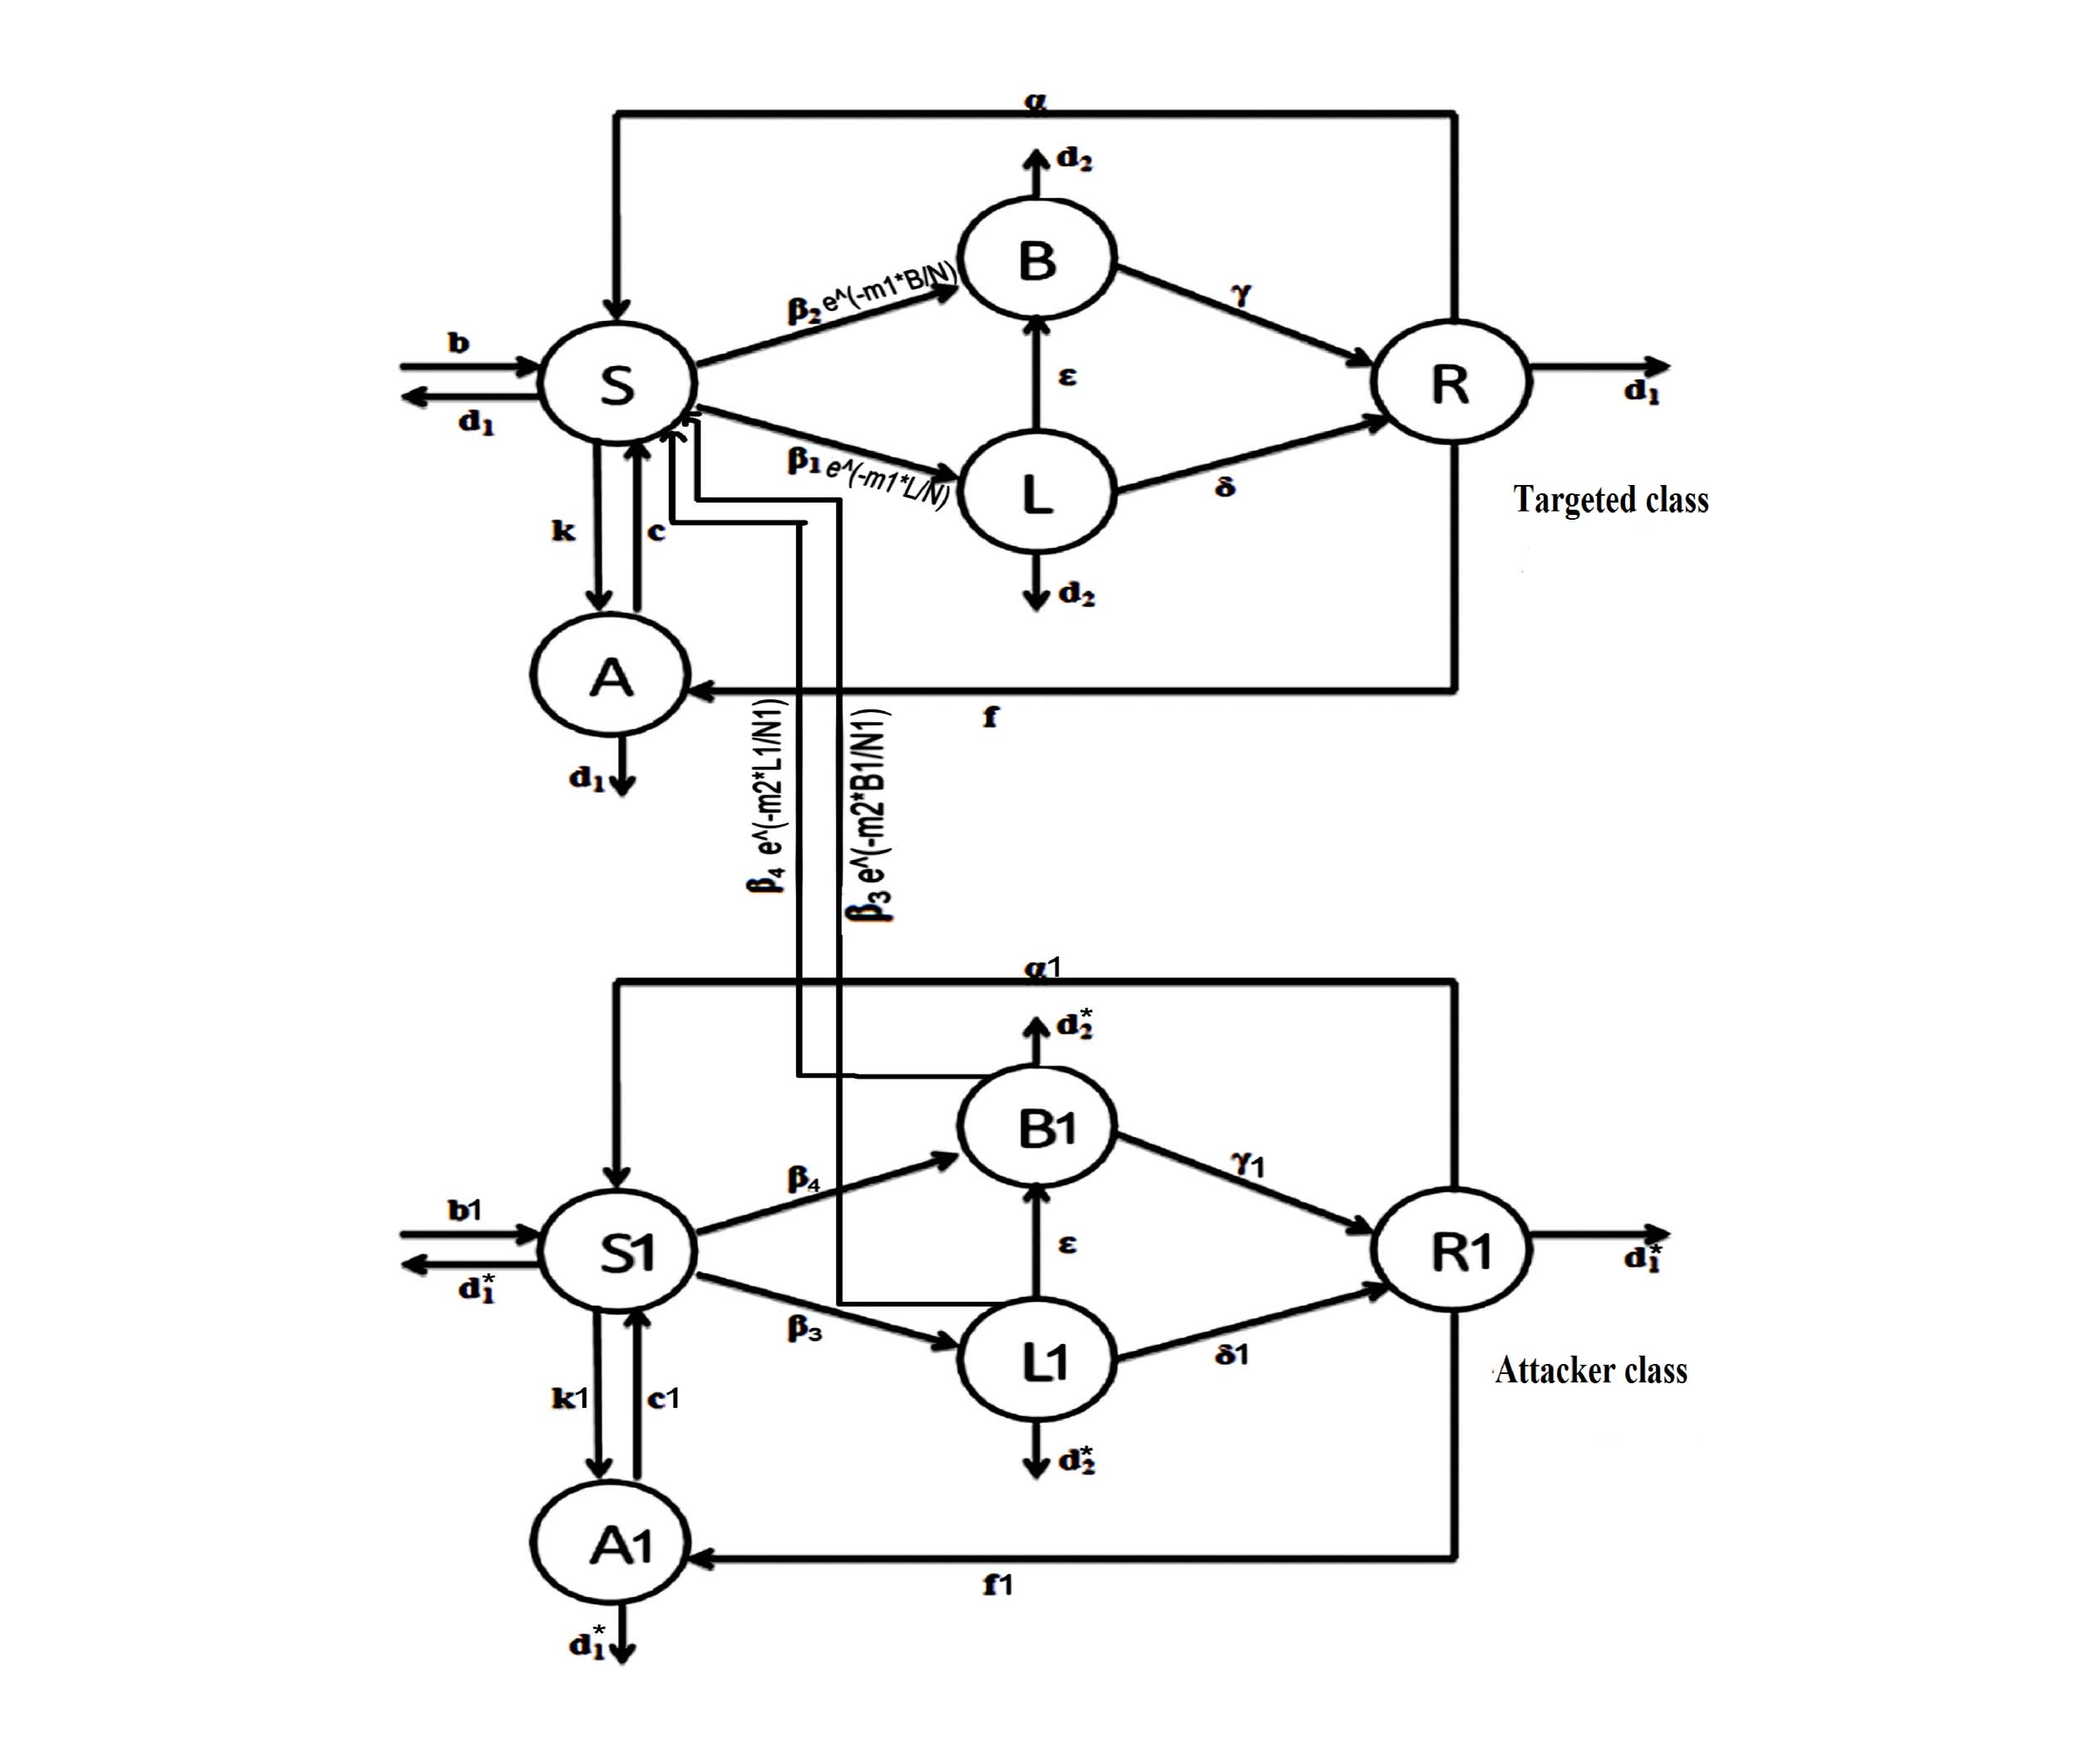
\includegraphics[width=1\columnwidth, clip=true]{modelcopy1.eps}
  \caption{Schematic Flow of Proposed Model}\label{sf1}
  %\end{minipage}
 \end{figure}
\newpage

\section{Mathematical Model}
Keeping in view the transmission rates of the schematic flow diagram which is shown in the figure \ref{sf1}. The system is defined by following set of ordinary differential equations:

\noindent \textbf{For targeted nodes:}
\begin{eqnarray}
\frac{d\tilde{S}}{d\tilde{t}} &=& b-\tilde{\beta_2} e^{-m_1 \frac{\tilde{B}}{\tilde{N}}}\tilde{S} \frac{\tilde{B}}{\tilde{N}}-\tilde{\beta_1} e^{-m_1\frac{\tilde{L}}{\tilde{N}}} \tilde{S}\frac{\tilde{L}}{\tilde{N}}-\tilde{k}\tilde{S}\tilde{A}+\tilde{c}\tilde{A}-\tilde{d_1}\tilde{S} \nonumber \\
&+&\tilde{\alpha} \tilde{R}-\tilde{\beta_2} e^{-m_2 \frac{\tilde{B_1}}{\tilde{N_1}}} \tilde{S} \frac{\tilde{B_1}}{\tilde{N_1}} -\tilde{\beta_1} e^{-m_2 \frac{\tilde{L_1}}{\tilde{N_1}}} \tilde{S} \frac{\tilde{L_1}}{\tilde{N_1}},
\label{se1}
\end{eqnarray}
\be
\frac{d\tilde{B}}{d\tilde{t}}=\tilde{\beta_2} e^{-m_1 \frac{\tilde{B}}{\tilde{N}}} \tilde{S}\frac{\tilde{B}}{\tilde{N}}-\tilde{d_2}\tilde{B}+\tilde{\epsilon} \tilde{L}-\tilde{\gamma} \tilde{B}+\tilde{\beta_2} e^{-m_2\frac{\tilde{B_1}}{\tilde{N_1}}}\tilde{S}
\frac{\tilde{B_1}}{\tilde{N_1}},
\label{se2}
\ee
\be
\frac{d\tilde{L}}{d\tilde{t}}=\tilde{\beta_1} e^{-m_1\frac{\tilde{L}}{\tilde{N}}} \tilde{S}\frac{\tilde{L}}{\tilde{N}}-\tilde{d_2}\tilde{L}-\tilde{\epsilon}\tilde{L}-\tilde{\delta} \tilde{L}+
\tilde{\beta_1} e^{-m_2\frac{\tilde{L_1}}{\tilde{N_1}}}\tilde{S}\frac{\tilde{L_1}}{\tilde{N_1}},
\label{se3}
\ee
\be
\frac{d\tilde{R}}{d\tilde{t}}=\tilde{\gamma} \tilde{B}+\tilde{\delta}\tilde{L}-\tilde{f}\tilde{R}-\tilde{\alpha} \tilde{R}-\tilde{d_1}\tilde{R},
\label{se4}
\ee
\be
\frac{d\tilde{A}}{d\tilde{t}}=\tilde{f}\tilde{R}-\tilde{d_1}\tilde{A}+ \tilde{k} \tilde{S}\tilde{A}-\tilde{c}\tilde{A}.
\label{se5}
\ee
\noindent\textbf{For attacker nodes:}\\
\be
\frac{d\tilde{S_1}}{d\tilde{t}}=b_1-\tilde{\beta_4}\tilde{S_1}\tilde{B_1} -\tilde{\beta_3} \tilde{S_1}\tilde{L_1}-\tilde{k_1} \tilde{S_1}\tilde{A_1}+\tilde{c_1}\tilde{A_1}-\tilde{d_3}S_1+\tilde{\alpha_1}\tilde{R_1},
\ee
\be
\frac{d\tilde{B_1}}{d\tilde{t}}=\tilde{\beta_4}\tilde{S_1}\tilde{B_1}-\tilde{d_4}\tilde{B_1}+\tilde{\epsilon_1}L_1-\tilde{\gamma_1}{B_1},
\ee
\be
\frac{d\tilde{L_1}}{d\tilde{t}}=\tilde{\beta_3}\tilde{S_1}\tilde{L_1}-\tilde{d_4}\tilde{L_1}-\tilde{\epsilon_1}L_1-\tilde{\delta_1}{L_1},
\ee
\be
\frac{d\tilde{R_1}}{d\tilde{t}}=\tilde{\gamma_1} \tilde{B_1} + \tilde{\delta_1}\tilde{L_1}-\tilde{f_1}\tilde{R_1}-\tilde{\alpha_1} \tilde{R_1}-\tilde{d_3}\tilde{R_1},
\ee
\be
\frac{d\tilde{A_1}}{d\tilde{t}}=\tilde{f_1}\tilde{R_1}-\tilde{d_3}\tilde{A_1}+\tilde{k_1}\tilde{S_1}\tilde{A_1}-\tilde{c_1}\tilde{A_1}.
\ee
where all the system parameters are positive and described in table \ref{table1}.
\begin{center}
\begin{table}
\scriptsize
\footnotesize
\begin{tabular}{|c|l|}
  \hline
  % after \\: \hline or \cline{col1-col2} \cline{col3-col4} ...
  \textbf{Parameters} & \textbf{Description }\\
  \hline
  $b,b_1$ & Recruitment rates\\
  \hline
  $d_1,d_2$ & Natural death rate of attacker and targeted population nodes\\
  \hline
  $\beta_1,\beta_3$ & Contact rate from susceptible class to latent class;(in the absence of firewall security) \\
  \hline
  $\beta_2,\beta_4$ & Contact rate from susceptible class to breaking-out class;(in the absence of firewall security) \\
  \hline
  $\gamma,\gamma_1$ & Rate of recovery of computers with malicious codes in breaking-out state \\
  \hline
  $\delta,\delta_1$ & Rate of recovery of computers with malicious codes in latent state \\
  \hline
  $d_3,d_4$ & Death rate in infected class(death due to infection and natural death) \\
  \hline
  $\epsilon,\epsilon_1$& Conversion rate of malicious codes from latent to braking-out state\\
  \hline
  $f,f_1$ & Conversion rate of recovered nodes into antidotal nodes \\
  \hline
  $c,c_1$ & Conversion rate of antidotal nodes into susceptible nodes \\
  \hline
  $k,k_1$ & Conversion rate of susceptible nodes into antidotal nodes \\
  \hline
  $\alpha,\alpha_1$ & Conversion rate of recovered nodes into susceptible nodes \\
  \hline
  $m_1, \ m_2$ & Firewall security coefficients\\
  \hline
\end{tabular}
\caption{Parameters Description}\label{table1}
\end{table}
\end{center}


\noindent Non-dimensionalise the above system using,

\noindent
$S=\frac{\tilde{S}}{\tilde{N}}$, $B=\frac{\tilde{B}}{\tilde{N}}$, $L=\frac{\tilde{L}}{\tilde{N}}$, $R=\frac{\tilde{R}}{\tilde{N}}$,
$A=\frac{\tilde{A}}{\tilde{N}}$, $S_1=\frac{\tilde{S_1}}{\tilde{N_1}}$, $B_1=\frac{\tilde{B_1}}{\tilde{N_1}}$, $L_1=\frac{\tilde{L_1}}{\tilde{N_1}}$,
$R_1=\frac{\tilde{R_1}}{\tilde{N_1}}$, $A_1=\frac{\tilde{A_1}}{\tilde{N_1}}$, $t=\tilde{d_1}\tilde{t}$, $N=\frac{\tilde{N}}{\tilde{N^0}}$,
$N_1=\frac{\tilde{N_1}}{\tilde{{N_1}^0}}$,$\tilde{N^0}=\frac{b}{\tilde{d_1}}$ and $\tilde{{N_1}^0}=\frac{b}{\tilde{d_3}}.$

\noindent The equivalent non-dimensional system is given by:

\noindent\textbf{For targeted nodes:}
\begin{eqnarray}
\frac{dS}{dt} &=& \frac{(1-S)}{N}-\beta_2 e^{-m_1B} SB-\beta_1 e^{-m_1L} SL-k SAN + cA - S + \alpha R  \nonumber\\
  &-&\beta_2 e^{-m_2B_1} SB_1-\beta_1 e^{-m_2L_1} SL_1+S^2+d_2SL+d_2SB+RS+AS,
\end{eqnarray}
\begin{eqnarray}
\frac{dB}{dt} &=& \beta_2 e^{-m_1B} SB-d_2B+\epsilon L-\gamma B+\beta_2 e^{-m_2B_1} SB_1-\frac{B}{N}+BS+d_2B^2 \nonumber\\
  &+&d_2BL+BR+BA,
\end{eqnarray}
\begin{eqnarray}
\frac{dL}{dt} &=& \beta_1 e^{-m_1L} SL-d_2L-\epsilon L-\delta L+\beta_1 e^{-m_2L_1} SL_1-\frac{L}{N}+SL \nonumber\\
  &+&d_2L^2+d_2BL+RL+AL,
\end{eqnarray}
\begin{eqnarray}
\frac{dR}{dt} &=& \gamma B+\delta L-fR-\alpha R-R-\frac{R}{N}+RS+d_2RB+d_2RL+R^2+RA,
\end{eqnarray}
\begin{eqnarray}
\frac{dA}{dt} &=& fR-A-cA+kASN-\frac{A}{N}+AS+d_2AB+d_2AL+AR+A^2.
\end{eqnarray}
\noindent\textbf{For attacker nodes:}
\begin{eqnarray}
\frac{dS_1}{dt}&=&\frac{(1-S_1)}{N_1}-\beta_4 S_1 B_1 N_1-\beta_3 S_1 L_1 N_1+c_1A_1-k_1 S_1A_1N_1-S_1+\alpha_1R_1 \nonumber \\
   &+&S_1^2+d_3S_1B_1+d_3S_1L_1+S_1R_1+S_1A_1,
\end{eqnarray}
\begin{eqnarray}
\frac{dB_1}{dt}&=&\beta_4S_1B_1N_1-d_3B_1+\epsilon_1L_1-\gamma_1B_1-\frac{B_1}{N_1}+B_1S_1+d_3{B_1}^2+d_3B_1L_1 \nonumber \\
   &+&B_1R_1+B_1A_1,
\end{eqnarray}
\begin{eqnarray}
\frac{dL_1}{dt}&=&\beta_3S_1L_1N_1-d_3L_1-\epsilon_1L_1-\delta_1L_1-\frac{L_1}{N_1}+S_1L_1+d_3{L_1}^2+d_3B_1L_1 \nonumber \\
   &+&R_1L_1+A_1L_1,
\end{eqnarray}
\begin{eqnarray}
\frac{dR_1}{dt}&=&\gamma_1B_1+\delta_1L_1-f_1R_1-\alpha_1R_1-R_1-\frac{R_1}{N_1}+R_1S_1+d_3R_1B_1+d_3R_1L_1 \nonumber \\
   &+&{R_1}^2+R_1A_1,
\end{eqnarray}
\begin{eqnarray}
\frac{dA_1}{dt}&=&f_1R_1-A_1-c_1A_1+k_1A_1S_1N_1-\frac{A_1}{N_1}+A_1S_1+d_3A_1B_1+d_3A_1L_1 \nonumber \\
   &+&A_1R_1+{A_1}^2.
\end{eqnarray}

\noindent Where targeted nodes and attacker nodes parameters are dimensionalised by $\tilde{d_1}$ and $\tilde{d_3}$ respectively.


\section{Boundedness of the System}

To verify our system is bounded, we classify the boundedness of the system into two parts , i.e., one for targeted  and other for attacker nodes.
For targeted population we define,
$$\tilde{N}(\tilde{t}) = \tilde{S}(\tilde{t}) + \tilde{L}(\tilde{t}) + \tilde{B}(\tilde{t}) + \tilde{R}(\tilde{t}) + \tilde{A}(\tilde{t}),$$
then,
$$\frac{d\tilde{N}}{d\tilde{t}}=\frac{d\tilde{S}}{d\tilde{t}}+\frac{d\tilde{L}}{d\tilde{t}}+\frac{d\tilde{B}}{d\tilde{t}}+\frac{d\tilde{R}}{d\tilde{t}}+\frac{d\tilde{A}}{d\tilde{t}},$$
$$\frac{d\tilde{N}}{d\tilde{t}}=b - \tilde{d_1}\tilde{S}-\tilde{d_2}\tilde{B}-\tilde{d_2}\tilde{L}-\tilde{d_1}\tilde{R}-\tilde{d_1}\tilde{A}.$$
Again, let
$$d =  {\text{min} \left\{\tilde{d_1},\ \tilde{d_2}\right\}},$$ then,
$$\frac{d\tilde{N}}{d\tilde{t}}\leq b- d[\tilde{S} + \tilde{L} + \tilde{B} + \tilde{R} + \tilde{A}]=b-d\tilde{N}.$$
If $\tilde{N}(\tilde{t}) > (b/d),$ then $\frac{d\tilde{N}}{d\tilde{t}} < 0$, implying $lim sup_{t \to \infty} \tilde{N}(\tilde{t}) \leq \frac{b}{d}$. After a moment of reflection, it can be seen that, for arbitrarily small $k>0$, simply connected compact set
$${\Omega}_k = \{(\tilde{S}, \tilde{L}, \tilde{B}, \tilde{R}, \tilde{A}) \in {R_{+}}^5: \tilde{S} + \tilde{L} + \tilde{B} + \tilde{R} + \tilde{A} \leq \frac{b}{d} + k\},$$
is positively invariant for this model. Hence, our proposed system is well posed. \\
Similarly we can define boundedness for the Attacker population.
$$\frac{d\tilde{N_1}}{d\tilde{t}}=b_{1} - \tilde{d_3}\tilde{S_{1}}-\tilde{d_{4}}\tilde{B_{1}}-\tilde{d_{4}}\tilde{L_{1}}-\tilde{d_{3}}\tilde{R_{1}}-\tilde{d_{3}}\tilde{A_{1}}.$$
Again, let
$$d_{1} =  {\text{min} \left\{\tilde{d_3},\ \tilde{d_4}\right\}},$$ then,
$$\frac{d\tilde{N_{1}}}{d\tilde{t}}\leq b_{1}- d_{1}[\tilde{S_{1}} + \tilde{L_{1}} + \tilde{B_{1}} + \tilde{R_{1}} + \tilde{A_{1}}]=b_{1}-d_{1}\tilde{N_{1}}.$$
If $\tilde{N_1}(\tilde{t}) > \frac{b_1}{d_1},$ then $\frac{d\tilde{N_1}}{d\tilde{t}} < 0$, implying $lim sup_{t \to \infty} \tilde{N_1}(\tilde{t}) \leq \frac{b_1}{d_1}$. After a moment of reflection, it can be seen that, for arbitrarily small $k_1>0$, simply connected compact set
$${\Omega}_{k_1} = \{(\tilde{S_{1}}, \tilde{L_{1}}, \tilde{B_{1}}, \tilde{R_{1}}, \tilde{A_{1}}) \in {R_{+}}^5: \tilde{S_{1}} + \tilde{L_{1}} + \tilde{B_{1}} + \tilde{R_{1}} + \tilde{A_{1}} \leq \frac{b_{1}}{d_{1}} + k_{1}\}.$$


































